%!TEX root = /Users/andy/Documents/Academics/Dissertation/thesis.tex
 %!TEX root = /Users/andy/Documents/Academics/Dissertation/thesis.tex

%\begin{savequote}[75mm] 
%It is well known that a discovery is simply the joining of two or more pieces of information to a useful end.
%\qauthor{Ramon y Cajal, \citep{cajal_advice_1999}} 
%\end{savequote}


\chapter{Optogenetic manipulation of neural activity in freely moving \textit{Caenorhabditis elegans}}\label{chapter:colbert}



\section{Introduction}
\lettrine{R}{easerchers in systems neuroscience} aim to understand how neural dynamics create behavior. Optogenetics has accelerated progress in this area by making it possible to stimulate or inhibit neurons that express light-activated proteins like channelrhodopsin-2 (ChR2) and halorhodopsin (also known as Halo/NpHR) by illuminating them \citep{nagel_channelrhodopsin-2_2003, boyden_millisecond-timescale_2005, zhang_channelrhodopsin-2_2006, han_multiple-color_2007,szobota_remote_2007,zhang_multimodal_2007,chow_high-performance_2010}. 
The nematode \textit{C. elegans} is particularly amenable to optogenetics due to its optical transparency, compact nervous system and ease of genetic manipulation \citep{nagel_light_2005, liewald_optogenetic_2008, guo_optical_2009,stirman_high-throughput_2010}.

The ability to deliver light to one cell with spatial selectivity is essential for targeted optogenetic perturbation in \textit{C. elegans} for the many cases where genetic methods do not provide adequate specificity. In the worm motor circuit, for example, there are no known single neuron-specific promoters that would drive expression of light-activated proteins in only one or a few neurons of the ventral nerve cord (VNC).
Optogenetics has been applied to the mechanosensory circuit in \textit{C. elegans}, but only through simultaneous stimulation of all touch receptor neurons because promoters specific to each neuron are unavailable \citep{nagel_channelrhodopsin-2_2003}. 
Researchers can use laser killing to study the contribution of single touch receptor neurons to overall behavior by removing neurons, but it is often preferable to work with intact circuits \citep{chalfie_neural_1985, wicks_dynamic_1996, kitamura_contribution_2001}.

Recently, a digital micromirror device (DMD) has been used to deliver light with high spatial selectivity in immobilized \textit{C. elegans} and immobilized \textit{Danio rerio} zebrafish \citep{wyart_optogenetic_2009}. Each element of a DMD may be independently controlled to deliver light to a corresponding pixel of a microscope's field of view. 
In many cases, however, the normal operation of neural circuits can be studied only in freely behaving animals, requiring a more sophisticated instrument.

Here we describe an optogenetic illumination system that allows perturbations of neural activity with high spatial and temporal resolution in an unrestrained worm, enabling us to \emph{Co}ntrol \emph{L}ocomotion and \emph{Be}havior in \emph{R}eal \emph{T}ime (CoLBeRT) in \textit{C. elegans}. In the CoLBeRT system, a video camera follows a worm under dark-field illumination while a motorized stage keeps the worm centered in the camera's field of view. Machine-vision algorithms estimate the coordinates of targeted cells within the worm body and generate an illumination pattern that is projected onto the worm by a DMD with laser light. The cycle repeats itself for each subsequent frame. Because the worm is a moving target, the faster an image can be captured and translated into DMD directives, the more accurately an individual cell can be targeted. The CoLBeRT system carries out all of these functions in \textasciitilde20 ms, providing a spatial resolution of \textasciitilde30 \textmu m in optogenetic control for freely swimming \textit{C. elegans}. We analyzed the motor circuit and mechanosensory circuit of unrestrained worms, demonstrating the performance of the CoLBeRT system, a new tool that enhances the flexibility and power of optogenetic approaches in \textit{C. elegans}.

\section{Results}
\subsection{Experimental Setup}
To stimulate neurons using ChR2 or inhibit neurons using Halo/NpHR, we used a 473-nm or 532-nm wavelength diode-pumped solid state (DPSS) laser, respectively  (Fig.~\ref{fig:colbert1}a). Either laser was incident onto a DMD with 1,024 × 768 elements. Laser light was reflected onto the specimen only when an individual micromirror was turned to the `on' position. We illuminated the specimen under dark-field illumination by red light to avoid exciting ChR2 or Halo/NpHR. Filter cubes reflected the wavelengths for optogenetic illumination from the DMD onto the sample, while passing longer wavelengths for dark-field illumination to a camera. A motorized stage kept the specimen in the field of view.


\begin{FPfigure} 
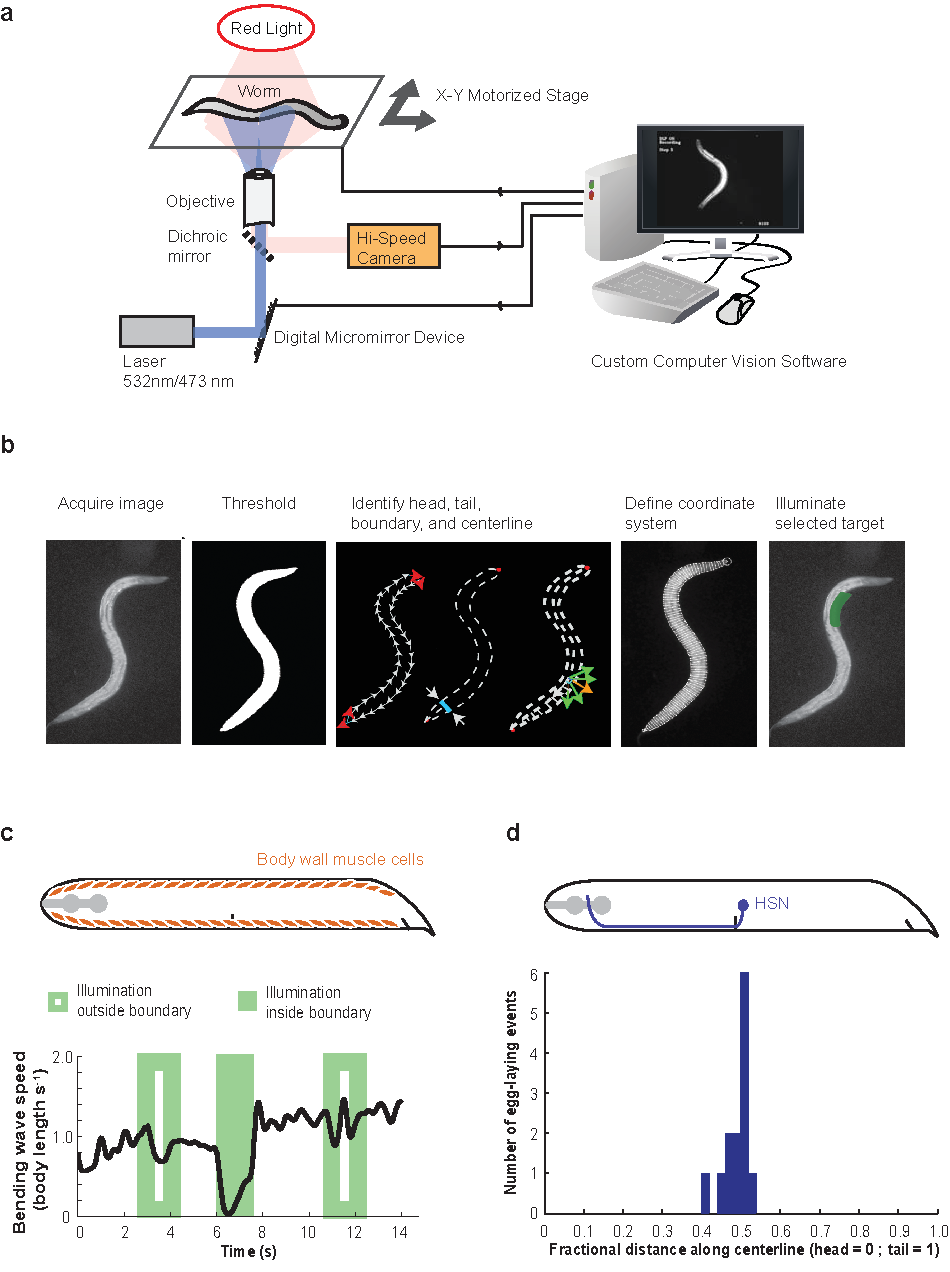
\includegraphics[width=\textwidth]{figures/colbert1}
\caption[CoLBeRT system apparatus and methodology]{High-resolution optogenetic control of freely moving \textit{C. elegans}.  (\textbf{a}) An individual worm swims or crawls on a motorized stage under red dark-field illumination. A high-speed camera images the worm. Custom software instructs a DMD to reflect laser light onto targeted cells. (\textbf{b}) Images are acquired and processed at ~50 FPS. Each 1,024 × 768 pixel image is thresholded and the worm boundary is found. Head and tail are located as maxima of boundary curvature (red arrows). Centerline is calculated from the midpoint of line segments connecting dorsal and ventral boundaries (blue bar) and is resampled to contain 100 equally-spaced points. The worm is partitioned into segments by finding vectors (green arrows) from centerline to boundary, and selecting one that is most perpendicular to the centerline (orange arrow). Targets defined in worm coordinates are transformed into image coordinates and sent to the DMD for illumination (green bar). (\textbf{c}) Schematic of body-wall muscles. Anterior, to left; dorsal, to top. Bending wave speed of swimming worm expressing Halo/NpHR in its body-wall muscles subjected to green light (10~mW~mm$^{-2}$) outside or inside the worm boundary (n = 5 worms, representative trace). (\textbf{d}) Schematic of HSN. A swimming worm expressing ChR2 in HSN was subjected to blue light (5~mW~mm$^{-2}$). Histogram, position at which egg-laying occurred when a narrow stripe of light was slowly scanned along the worm's centerline (n = 13 worms). Once an egg was laid, the worm was discarded. \label{fig:colbert1}}
\end{FPfigure}
\afterpage{\clearpage}


To accelerate real-time image analysis of worm posture, we developed the MindControl software package using the open-source OpenCV computer vision library\citep{bradski_opencv_2000}. With the graphical user interface (GUI), the user can dynamically target specific regions of freely moving worms. The MindControl software and documentation are available at \href{http://github.com/samuellab/mindcontrol}{http://github.com/samuellab/mindcontrol}.


The MindControl software carries out a sequence of image analysis operations on each frame received from the camera (Fig.~\ref{fig:colbert1}b). An image is captured by the computer, filtered and thresholded. Next, the boundary of the worm is calculated, and head and tail are identified as local maxima of boundary curvature (the head is blunt and the tail is sharp). The worm centerline is calculated and the body is divided into 100 evenly-spaced segments. These segments define a worm coordinate system invariant to worm posture or orientation, within which the user may define target positions. The software maps the position of targets onto the coordinates of the real image and, finally, sends the appropriate pattern to the DMD for illumination.

For our current system, the total latency between image acquisition and DMD illumination is 20~ms: image exposure, 2~ms; data transfer to computer, 3~ms; image analysis, 10~ms; and data transfer to DMD, 5~ms. Given the size and speed of a swimming worm at 10× magnification, our system working at \textasciitilde50 frames per second (FPS) delivers optogenetic illumination with a spatial resolution of \textasciitilde30~\textmu m, not far from the spatial resolution limit imposed by the pixel density of the DMD (\textasciitilde5~\textmu m at 10× magnification).

\subsection{Spatial resolution of the illumination system}
First, we confirmed that illumination is restricted to the targeted area. We examined a transgenic worm expressing \textit{Halo/NpHR::CFP} in all body-wall muscles. Whole-animal illumination of transgenic P\textit{myo-$3$::Halo/NpHR} worms causes all muscles to relax \citep{zhang_multimodal_2007}. We placed individual swimming worms in the CoLBeRT system and used green light (532 nm, 10~mW~mm$^{-2}$) to alternately illuminate the entire region outside or inside the worm boundary (Fig.~\ref{fig:colbert1}b and Video \ref{movie:colbert1}). Illuminating the entire region outside the worm boundary had no effect-- the bending waves propagated from head to tail at normal speed. Illuminating the entire region inside the worm boundary, however, arrested locomotion--- the body relaxed and the speed of bending waves dropped to zero.

To quantify the spatial resolution of the CoLBeRT system, we measured its targeting accuracy in evoking egg-laying events by stimulating the HSN motor neurons. We used transgenic worms expressing ChR2 under the \textit{egl-$6$} promoter, which drives expression in the bilaterally symmetric HSN neurons (HSNL and HSNR) as well as glia-like cells in the worm's head  \citep{ringstad_fmrfamide_2008}. Optogenetic stimulation of the HSN neurons, which innervate the vulval musculature, evokes egg-laying behavior (L. Emtage and N. Ringstad, personal communication).

The two HSN neurons lie on top of one another when the worm is viewed laterally, so our system targets both neurons. We projected a thin stripe of blue light (473 nm, 5~mW~mm$^{-2}$) on the body of swimming P\textit{egl-6d::ChR2} transgenic worms. The long axis of the stripe was orthogonal to the worm centerline and spanned its diameter. The stripe width corresponded to 2\% of the anterior-posterior length of the worm centerline (that is, \textasciitilde20 \textmu m of the \textasciitilde1-mm-long young adult worm). We used narrow stripes so that our illumination would  less likely stimulate HSN when illuminating its process. We slowly moved the illumination stripe along the centerline of swimming worms while recording egg-laying events. Of 14 worms studied, we observed 13 egg-laying events, eight in which the stripe started at the head and five in which the stripe started at the tail. Egg-laying frequency sharply peaked when the center of the stripe coincided with the centerline coordinate of the HSN cell bodies, or 49.6\% of the total distance from the anterior to the posterior of the body with 3.2\% s.d. (Fig.~\ref{fig:colbert1}d and Video \ref{movie:colbert2}). The width of this distribution suggests that the CoLBeRT system provides at least \textasciitilde30 \textmu m of spatial resolution.


\subsection{Optogenetic manipulation of muscle cells}
In \textit{C. elegans}, forward movement is driven by motor neurons in the VNC, which coordinate the activity of 95 body wall muscle cells along the dorsal and ventral sides of the VNC \citep{von_stetina_motor_2006}. The circuit for worm locomotion is poorly understood in comparison to that of other undulatory animals such as the leech and lamprey \citep{marder_principles_1996, bryden_neural_2008, karbowski_systems_2008}. Because this circuit probably operates normally only during normal movement, technology such as the CoLBeRT system is necessary to dissect cellular activity in unrestrained animals.

We used the CoLBeRT system to suppress muscle activity in a region of the body in P\textit{myo-$3$ ::Halo/NpHR::CFP} transgenic worms (Fig.~\ref{fig:colbert2} and Video \ref{movie:colbert3}). This perturbation of undulatory dynamics can be shown graphically using a red-blue color map to represent the curvature of the body centerline in nondimensional units (that is, the curvature calculated at each point along the centerline, $\kappa$, multiplied by worm length, $L$) as a function of time and fractional distance along the centerline, $s$, from head ($s = 0$) to tail ($s = 1$) (Fig.~\ref{fig:colbert2}a). Notably, hyperpolarizing muscle cells in one segment had no effect on undulatory dynamics anterior to the segment, but lowered the amplitude of the bending wave posterior to the illuminated segment (Fig.~\ref{fig:colbert2}b). Representative data from one of five worms that we studied are shown in Figure \ref{fig:colbert2}. Thus, the bending of posterior body segments seems coupled to the bending of anterior body segments. One possibility is that muscle activity in posterior segments is directly promoted by muscle activity in anterior segments, perhaps by gap junction coupling between muscle cells \citep{liu_low_2006}. Another possibility is that the motor circuit contains a proprioceptive mechanism that makes the activity of posterior segments directly sensitive to the bending of anterior segments.

\begin{figure} 
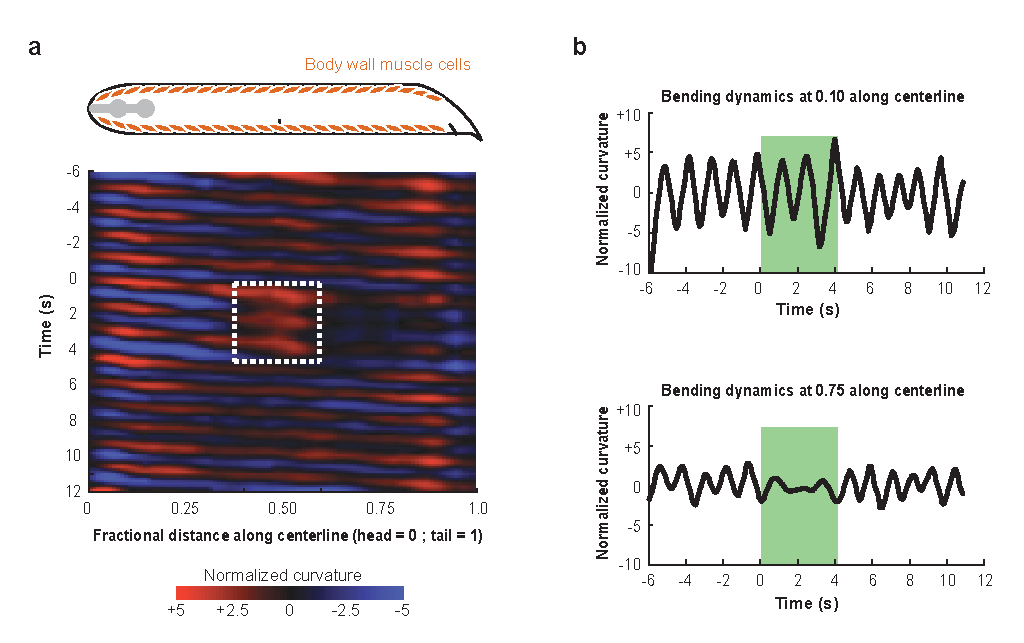
\includegraphics[width=\textwidth]{figures/colbert2}
\caption[Optogenetic inactivation of muscle cells.]{Optogenetic inactivation of muscle cells. (\textbf{a}) Kymograph of time-varying body curvature along the centerline of a P\textit{myo-$3$::Halo/NpHR::CFP} transgenic worm. Between 0 s and 4 s, the worm was illuminated with green light (10~mW~mm$^{-2}$) in a region spanning the worm diameter and between 0.38 and 0.6 of the fractional distance along the centerline. (\textbf{b}) For the kymograph in \textbf{a}, time-varying curvature at two points along the worm centerline, both anterior (top) and posterior (bottom) to the illuminated region. \label{fig:colbert2}}
\end{figure}
\afterpage{\clearpage}

\subsection{Optogenetic manipulation of cholinergic motor neurons}
The cell bodies of motor neurons in \textit{C. elegans} are distributed along the VNC \citep{von_stetina_motor_2006,wicks_dynamic_1996}. Ventral muscles are innervated by the cholinergic VA, VB and VC motor neurons and GABAergic VD motor neurons. Dorsal muscles are innervated by the cholinergic DA, DB and AS motor neurons and GABAergic DD motor neurons\citep{white_structure_1976,chen_wiring_2006}. A current model is that VA and DA drive muscle contraction during backward locomotion, VB and DB drive muscle contraction during forward locomotion and VD and DD motor neurons drive muscle relaxation during both forward and backward locomotion \citep{wicks_dynamic_1996,von_stetina_motor_2006,haspel_motoneurons_2010}. A repeating motif of synaptic connectivity between the motor neurons runs along the worm body and allows for contralateral inhibition \citep{von_stetina_motor_2006}. During forward locomotion, for example, the DB (or VB) motor neurons can simultaneously excite a dorsal (or ventral) muscle cell while exciting the GABAergic VD (or DD) motor neurons that inhibit the opposing ventral (or dorsal) muscle cell \citep{white_structure_1976,chen_wiring_2006}. How this network drives the rhythmic undulatory wave, however, is poorly understood.

We analyzed the contributions of cholinergic neurons to forward locomotion using transgenic worms expressing Halo/NpHR in all cholinergic neurons under the control of the \textit{unc-17} promoter \citep{roghani_molecular_1994}. In P\textit{unc-17::Halo/NpHR::CFP} transgenic worms, illumination of a short segment of the VNC suppressed propagation of the undulatory wave to the entire region posterior to the illuminated segment without affecting the undulatory wave anterior to the illuminated segment (Fig.~\ref{fig:colbert3}a,b and Video \ref{movie:colbert4}). Representative data from one of five worms that we studied are shown in Figure \ref{fig:colbert3}a,b. This suggests that the activity of posterior VB and DB neurons is coupled to the activity of anterior VB and DB neurons, consistent with a wave of neuronal excitation that propagates from head to tail during forward movement.

\begin{figure} 
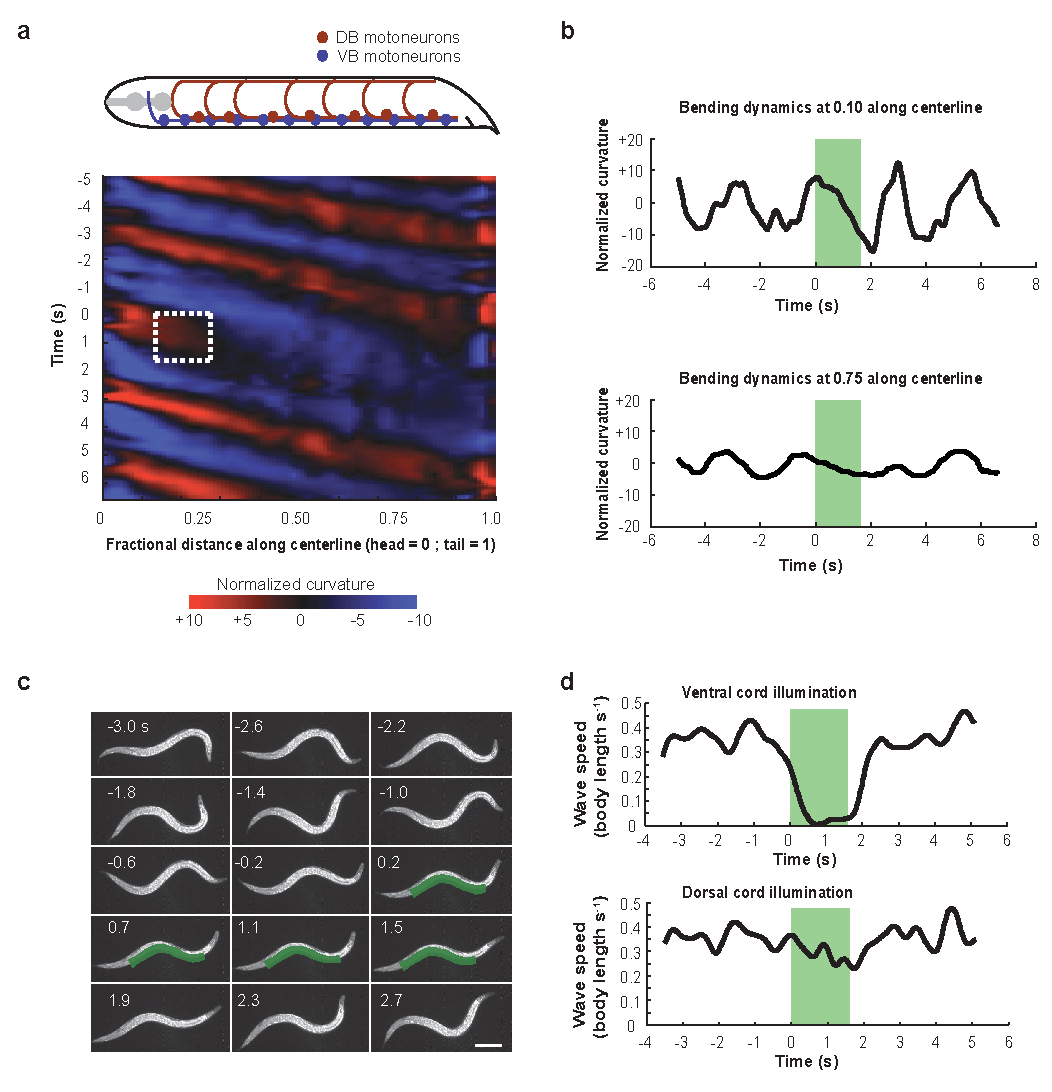
\includegraphics[width=\textwidth]{figures/colbert3}
\caption[Inhibition of motor neurons. ]{ Inhibition of motor neurons.  (\textbf{a}) Schematic of cholinergic DB and VB motor neurons. Anterior, to left; dorsal, to top. Kymograph of time-varying body curvature along the centerline of a P\textit{unc-17::Halo/NpHR::CFP} transgenic worm illuminated by a stripe of green light (10~mW~mm$^{-2}$) along its VNC between $t$ = 0 s and 1.6 s. In the dorsal-ventral direction, the stripe width was equal to 50\% of the worm diameter and centered on the ventral boundary. In the anterior-posterior direction, the stripe length was between 0.14 and 0.28 of the fractional distance along the body. (\textbf{b}) For the kymograph in a, time-varying curvature at two points along the worm centerline, both anterior (top) and posterior (bottom) to the illuminated region. (\textbf{c}) Video sequence of worm illuminated by a long stripe of green light (10~mW~mm$^{-2}$) spanning the VNC between $t$ = 0 s and 1.8 s. Scale bar, ~100 \textmu m. (\textbf{d}) Bending wave speed of a swimming worm illuminated by a long stripe of green light (10~mW~mm$^{-2}$) lasting 1.8 s and spanning the VNC (top) and dorsal nerve cord (bottom).\label{fig:colbert3}}
\end{figure}
\afterpage{\clearpage}

Using the CoLBeRT system, we can also specifically illuminate either the dorsal nerve cord or the VNC (Video \ref{movie:colbert5}). The VNC contains the cell bodies of the cholinergic motor neurons, whereas the dorsal nerve cord contains only nerve processes. Illuminating the entire VNC was particularly effective in hyperpolarizing the cholinergic motor neurons of P\textit{unc-17::Halo/NpHR::CFP} worms, inducing paralysis. Illuminating the entire dorsal nerve cord, however, produced only a small ( \textasciitilde15\%) drop in the speed of wave propagation (Fig.~\ref{fig:colbert3}c,d). The asymmetric effect of illuminating the ventral and dorsal nerve cords is probably due to the higher density of optogenetic protein in the cell bodies.

Surprisingly, the paralysis evoked by illuminating the VNC can occur without allowing relaxation of the worm body. In this instance, as long as the entire cholinergic network within the VNC was deactivated, the worm retained the posture it had immediately before illumination (Fig.~\ref{fig:colbert3}c). When the muscle cells of a swimming worm were hyperpolarized, on the other hand, the body straightened (Video \ref{movie:colbert1}). This observation suggests that muscle cells can remain in contracted or relaxed states without requiring continuous cholinergic input.


\subsection{Optogenetic manipulation of single touch receptor types}
Next, we applied the CoLBeRT system to the touch receptor system in \textit{C. elegans}. Six cells are specialized for sensing gentle touch in \textit{C. elegans}: the left and right anterior lateral microtubule cells (ALML and ALMR, respectively); the left and right posterior lateral microtubule cells (PLML and PLMR, respectively); the anterior ventral microtubule cell (AVM); and the posterior ventral microtubule cell (PVM) \citep{chalfie_neural_1985}. Gently touching the worm near its anterior stimulates reversal movement dependent on ALML, ALMR and AVM. Gently touching the worm near its posterior stimulates forward movement dependent on PLML and PLMR. The role of PVM remains unclear.

Channelrhodopsin can be expressed in all six touch receptor cells using the \textit{mec-4} promoter. Illuminating the whole body of transgenic worms with blue light evokes reversal responses, presumably by simultaneously activating ALM, AVM and PLM1. With the spatial resolution afforded by the CoLBeRT system, we could individually activate the ALM, AVM and PLM cell types. The left and right lateral cells (ALML and ALMR; PLML and PLMR) lie on top of one another when the worm is viewed laterally. Illuminating the anterior end containing both the AVM and ALM neurons triggered reverse movement (Fig. \ref{fig:colbert4}a and Video \ref{movie:colbert6}). Illuminating the posterior end containing the PLM neurons triggered forward movement (Fig. \ref{fig:colbert4}b and Video \ref{movie:colbert7}). Representative data from one of five worms that we studied are shown in Figure \ref{fig:colbert4}a,b.


\begin{FPfigure} 
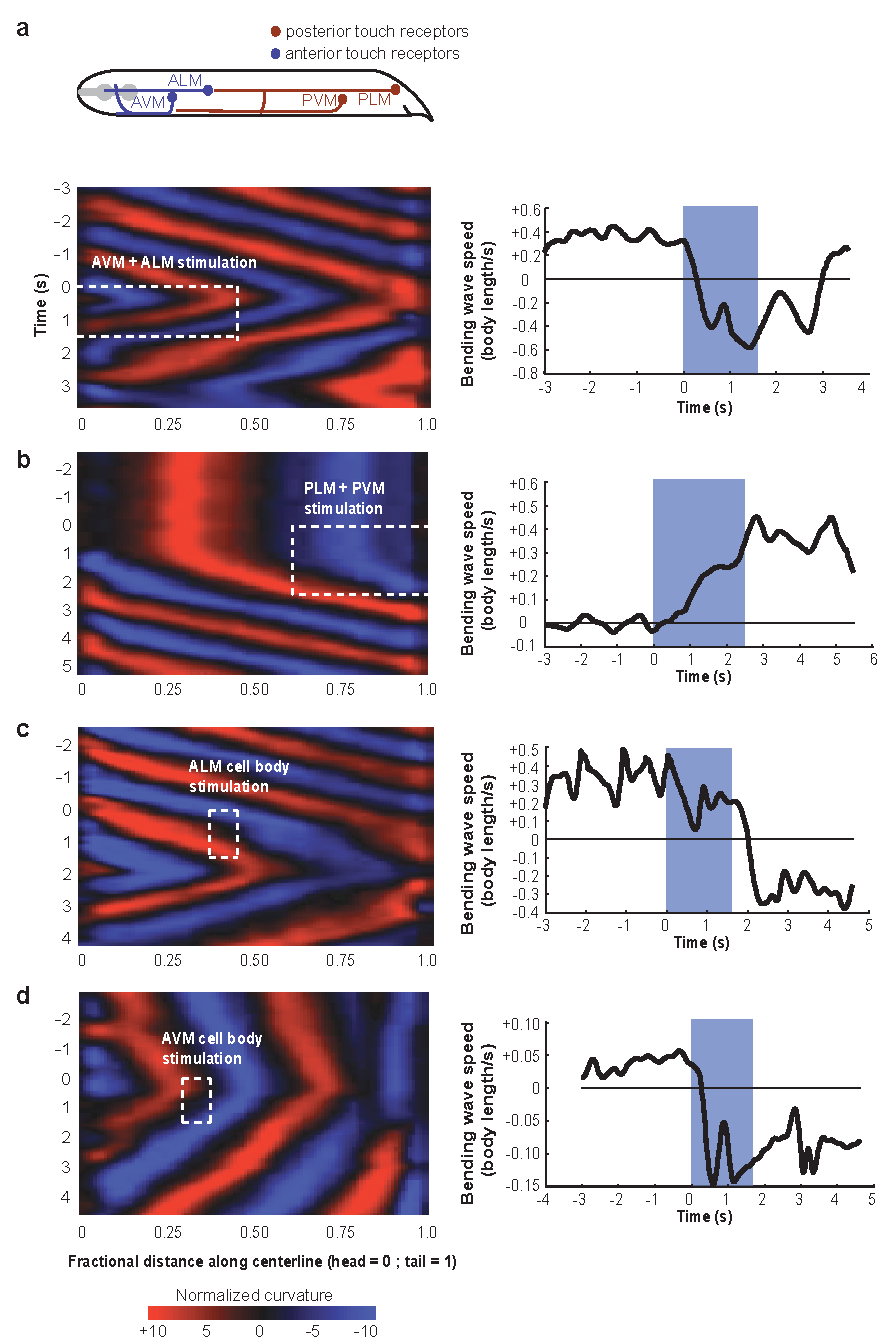
\includegraphics[width=\textwidth]{figures/colbert4}
\caption[Optogenetic analysis of mechanosensory neurons. ]{ Optogenetic analysis of mechanosensory neurons.  (\textbf{a})Top, schematic of anterior and posterior touch receptor cells. 
Anterior, to left; dorsal, to top. Kymographs (left) of time-varying curvature of centerline of worms expressing ChR2 in mechanosensory neurons (P\textit{mec-4::ChR2::GFP}) subjected to rectangles of blue light (5~mW~mm$^{-2}$) targeting different groups of touch receptor neurons. Plots of bending wave speed (right) indicate stimulus-evoked changes in direction or speed. AVM and ALM neurons are subjected to 1.5 s of stimulation. Given a coordinate system where $x$ specifies dorsal-ventral location (–1, dorsal boundary; 0, centerline; 1, ventral boundary) and $y$ defines fractional distance along the worm's centerline (0, head; 1, tail), the rectangle of illumination has corners ($x$,$y$) = ((-1.1,0),(1.1,0.46)). 
(\textbf{b}) PVM and PLM neurons are subjected to 2.5 s of stimulation with a rectangular illumination ($n$ = 5 worms, representative trace) with corners at ($x$,$y$) = ((-1.1,0.62),(1.1,0.99)). (\textbf{c}) ALM cell body is specifically stimulated by illuminating a small rectangle with corners at ($x$,$y$) = ((-0.3,0.38), (-0.9,0.46)). 
(\textbf{d}) AVM cell body is specifically stimulated by illuminating a small rectangle with corners at ($x$,$y$) = ((0.3,0.3),(0.9,0.38)).\label{fig:colbert4}}
\end{FPfigure}
\afterpage{\clearpage}

Using the CoLBeRT system, we also induced reversals by targeting just AVM or ALM with an illumination box (20 \textmu m in the dorsal-ventral dimension; 30 \textmu m in the anterior-posterior direction for a young adult worm) that was centered on each cell body (Fig.~\ref{fig:colbert4}c,d and Videos \ref{movie:colbert8} and \ref{movie:colbert9}). Representative data from one of 14 worms that we studied are shown in Figure \ref{fig:colbert4}c,d. Using these illumination boxes, we could avoid illuminating the axon of the nontargeted neuron. These observations are consistent with earlier work showing that single touch receptor types are sufficient to drive behavioral responses \citep{chalfie_developmental_1981}.

To confirm that the CoLBeRT system can specifically target either AVM or ALM, we used transgenic worms expressing the photoconvertible fluorescent protein Kaede in the mechanosensory neurons \citep{ando_optical_2002}. Upon illumination by UV or violet light, Kaede converts from a green to red fluorescent state. We used the CoLBeRT  system with 405-nm light to specifically illuminate either the AVM or ALM cell bodies for 60 s in freely moving P\textit{mec-4::Kaede} worms. We found that worms in which AVM or ALM had been targeted showed only detectable red fluorescence in AVM or ALM, respectively, whereas all mechanosensory neurons showed green fluorescence (Fig.~\ref{fig:colbert5}a,b). When targeting ALM, a transient segmentation error owing to an omega turn by the worm caused the system to illuminate PLM and PVM for ~1 s, producing slight photoconversion in those neurons (Fig.~\ref{fig:colbert5}b). By quantifying the ratio between the red and green fluorescence signals, we estimated that the nontargeted neurons were illuminated for less than \textasciitilde1 s (Methods).

\begin{figure} 
\includegraphics[width=\textwidth]{figures/colbert5}
\caption[Habituation of individual touch receptor neuronal types.]{ Habituation of individual touch receptor neuronal types. (\textbf{a,b}) Schematic showing anterior and posterior touch receptor neurons (top). Anterior, to left; dorsal, to top. A freely swimming worm expressing Kaede in touch receptor neurons was continuously tracked and illuminated with a small rectangle of 405~nm light (2~mW~mm$^{-2}$) centered on either AVM or ALM (as in Fig.~\ref{fig:colbert4}c,d) for 60 s. Red and green fluorescence images are shown. Scale bars, 100~\textmu m. (\textbf{c–e}) Individual ALM and AVM neurons were repeatedly stimulated with blue light (5~mW~mm$^{-2}$) for 1.5 s every 60 s for \textasciitilde40 min, either alone (\textbf{c,d}) or interleaved within each experiment (\textbf{e}; ALM, 30 s; AVM, 30 s; ALM, 30 s; and so on). Fractional response to stimulus of each neuronal type was fit to an exponential, $a + b \exp(–t/\tau)$, using maximum likelihood estimator. Time constant for habituation, $\tau$, was extracted from each fit. Error bars, s.e.m. Fractional response of ALM when stimulated alone (\textbf{c}; $n$ = 7 worms). Fractional response of AVM when stimulated alone (\textbf{d}; $n$ = 8 worms). Fractional response of ALM (left) and AVM (right) during interleaved stimulation of both (\textbf{e} ; $n$ = 7 worms).\label{fig:colbert5}}
\end{figure}
\afterpage{\clearpage}


It has been shown that the mechanosensory circuit habituates to repetitive optogenetic stimulation \citep{nagel_light_2005}. We used the CoLBeRT system to quantify the rate of AVM and ALM habituation over 40 minuntes by repeatedly stimulating either AVM or ALM every 60 s. We observed comparable rates of habituation for both ALM and AVM (Fig.~\ref{fig:colbert5}c,d). Others have studied loci for habituation in the mechanosensory circuit by laser-killing touch receptor cells and/or downstream neurons and quantifying rates of habituation to gentle touch \citep{wyart_optogenetic_2009}. If habituation partly occurs at interneurons that are downstream of both ALM and AVM, then we might expect cross-habituation of the AVM response to repeated ALM stimulation, and vice versa. Cross-habituation may also be mediated by an electrical gap junction between AVM and ALM \citep{white_structure_1976}. To test whether cross-habituation occurs, we subjected a worm to interleaved AVM and ALM stimulation every 30 s, such that each neuron type was stimulated every 60 s. We found that the rates of habituation to both AVM and ALM stimulation were indeed more rapid with interleaved stimulation than with individual stimulation. This effect was particularly pronounced in the case of AVM stimulation (Fig.~\ref{fig:colbert5}e).

\section{Discussion}
At present, the spatial resolution of CoLBeRT is \textasciitilde{30} \textmu m when tracking a swimming worm. The system has better resolution when tracking the slower movements of a crawling worm, but is ultimately limited to \textasciitilde5~\textmu m resolution due to the pixel resolution of the DMD. Higher spatial resolution could be reached by tracking a specific region of the worm (for example, the nerve ring) at higher magnification. This modification to CoLBeRT would require a different approach to image analysis and targeting-- for example, analysis of cell body fluorescence instead of analysis of the posture of the whole worm.

CoLBeRT may be adapted to the opto\-gen\-etic analysis of other genetic\-ally tract\-able, trans\-parent animals such as the larvae of  \textit{Drosophila melanogaster} or \textit{D. rerio}. A simplified version of CoLBeRT may also be used to facilitate optogenetic illumination in other settings like studies of mammalian brain slices or exposed brain surfaces. Variants of CoLBeRT, using its capacity for rapid closed-loop feedback, may be used to trigger optogenetic stimulation based on simultaneous recordings of neural activity in addition to animal posture.

CoLBeRT is a flexible and easy-to-use platform for designing and projecting arbitrary spatiotemporal patterns of illumination with closed-loop sensitivity to the real-time behavior of the worm.

\section{Methods}
\subsection{Strains}
We cultivated transgenic worms in the dark at 20 \textdegree C on nematode growth medium (NGM) plates with OP50 bacteria with all-trans retinal. We made OP50-retinal plates by seeding 6-cm NGM plates with 250 $\mu$l of a suspension of OP50 bacteria in LB, to which we added 1 $\mu$l of 100~mM retinal in ethanol immediately before seeding. Plates were stored in the dark and all worms were handled in the dark or under red light.


Strain FQ10 (P\textit{egl-6::ChR2::YFP}) was a gift of Nials Ringstad. Strain QH3341 (vdEx128(P\textit{mec-4::Kaede})) was a gift of Brett Neu\-mann and Massimo Hill\-iard. Strains ZX444 (\textit{lin-15}(n765ts); zxEx29 (P\textit{myo-3::NpHR::ECFP}; \textit{lin-15}+)) and ZX422 (\textit{lin-15}(n765ts); zxEx33 (P\textit{unc-17::NpHR::ECFP}; \textit{lin-15}+)) were gifts of Alex\-ander Gotts\-chalk. Strain P\textit{myo-3::Halo::CFP} used in our experiments was generated by integrating the trans\-gene in ZX444 by cobalt-60 irradiation and outcrossing the resulting strain three times to the wild-type N2 strain. Strain P\textit{unc-17::Halo::CFP} used in our experiments was generated by Mei Zhen by irradiating ZX422 using UV radiation and outcrossing twice to the wild-type N2 strain. The P\textit{mec-4::ChR2} strain (QW309) was generated by injection of P\textit{mec-4::ChR2::YFP} plasmid at 100~ng~$\mu$l$^{-1}$ into \textit{lin-15}(n765ts) worms along with the \textit{lin-15} rescuing plasmid (pL15 EK) at 50~ng~$\mu$l$^{-1}$. The extrachromosomal array was integrated using gamma irradiation and outcrossed four times to wild-type N2.

\subsection{Microscopy}
The setup was built around a Nikon Eclipse TE2000-U inverted microscope. We carried out dark-field imaging using annular illumination of the specimen through a Ph3 phase ring. A filter transmitting red light (Hoya) was mounted to the microscope illumination optical pathway to minimize inadvertent activation of ChR2 or Halo/NpHR owing to dark-field illumination.

We imaged worms using a 10×, numerical aperture (NA) 0.45 Plan Apo objective. We used a custom optical system composed of two camera lenses (Nikon) to reduce the size of the image on the camera by a factor of 3.5. This allowed us to capture almost all of the 2.5-mm-diameter field of view on the camera sensor. We used a PhotonFocus MV2-D1280-640CL camera and BitFlow Karbon PCI Express ×8 10-tap Full Camera Link frame grabber to capture images.

The microscope stage was controlled by a Ludl BioPrecision2 XY motorized stage and MAC 6000 stage-controller. During data acquisition, computer software kept the worm centered in the field of view via an automated feedback loop.

\subsection{Optics and illumination} \label{colbert:opticsMetheds}
To stimulate ChR2, we used a DPSS laser (LP473-100, 473-nm wavelength, 100-mW maximum power, LaserShowParts). Similarly, to stimulate Halo/NpHR we used a DPSS laser (LP532-200, 532-nm wavelength, 200-mW maximum power, LaserShowParts). To photoconvert Kaede, we used a DPSS laser (EL-100B, 405-nm wavelength, 100-mW maximum power, Laserwold). The beams from the 473-nm and 532-nm lasers were aligned to a common path by a dichroic beamsplitter. The beam from the 405-nm laser was aligned to the common path with a retractable mirror. For each experiment, however, only one of the three lasers was used. The laser beam was expanded using a telescope composed of two plano-convex lenses and incident onto a 1,024 × 768 pixel digital micromirror device (Texas Instruments DLP, Discovery 4000 BD VIS 0.55-inch XGA, Digital Light Innovations) attached to a mirror mount. Using a series of mirrors, the laser was aligned so that the reflected beam for the `on' state of the DMD was centered on the optical axis of the illumination pathway.

The plane of the DMD was imaged onto the sample via the epifluorescence illumination pathway of the microscope using an optical system composed of two achromatic doublet lenses. We used a dichroic filter, FF580-FDi01-25x36 (Semrock), to reflect 405-nm, 473-nm or 532-nm laser light onto the sample while passing wavelengths used for dark-field illumination ($\lambda$ > 600 nm). We used an emission filter, BLP01-594R-25 (Semrock), to prevent stray laser reflections from reaching the camera. The dichroic and emission filters were mounted in a custom filter cube in the microscope filter turret.

\subsection{Software}
The microscope and all its components were controlled with custom MindControl software running Windows XP on an Acer Veriton M670G computer with an Intel Core 2 Quad processor running at 2.83 GHz with 3 GB of RAM. MindControl enables the user to define arbitrary illumination patterns for optogenetic stimulation, and to deliver illumination patterns either manually or automatically. For rapid operation, MindControl was written in the C programming language using the open-source OpenCV computer vision library, along with Intel's Integrated Performance Primitives for maximal speed. To further increase speed, we used multiple threads to separately handle image processing and the user interface. Every 20 ms, MindControl acquires an image from the camera, computes the location of the worm, generates an illumination pattern and sends that pattern to the DMD. 

For each video frame, the boundary and centerline of the worm and the status of the stimulus is recorded in a human- and computer-readable YAML file. Every frame is also recorded in two video streams, one containing annotations about optogenetic stimulation, and the other containing only images of the freely moving worm. A GUI allows the user to adjust the parameters of optogenetic stimulation in real time during each experiment. After each experiment, we used custom scripts written in Matlab to carry out quantitative analysis of the resulting video. All software and documentation is freely available for modification and redistribution under the GNU general public license. The software for optogenetic stimulis and analysis are available at \url{http://github.com/samuellab/mindcontrol} and  \url{http://github.com/samuellab/mindcontrol-analysis}, respectively.


\subsection{Behavioral experiments}

For motor circuit experiments, we washed each young adult worm in NGM solution before transferring it to a chamber composed of \textasciitilde100 $\mu$l of a 30\% dextran (wt/vol) in NGM solution sandwiched between two microscope slides separated by 0.127~mm. In this chamber, the worm was approximately confined to two dimensions but otherwise able to move freely. We then placed the chamber on the microscope for data collection.

To analyze egg-laying, we selected gravid adult worms, washed them in NGM and transferred them to chambers as described above. Each worm was subject to sequential pulses of 4~s of blue light illumination. Each pulse illuminated a stripe orthogonal to the worm centerline, spanning the worm diameter with width corresponding to 2\% of total body length. The stripe progressed along the worm centerline from head to tail or from tail to head until the first egg was laid. After an egg was laid, the trial ended and the worm was killed. Out of 14 worms studied, one did not lay any eggs.

For mechanosensory circuit experiments, we prescreened young adult P\textit{mec-4::ChR2} worms on a fluorescence stereo microscope (Nikon SMZ 1500) by illuminating the anterior of the worm with blue light from a 50-W mercury lamp through a GFP excitation filter. Only worms that responded with a reversal were chosen for further experiments. We carried out this prescreening procedure because the P\textit{mec-4::ChR2} strain (QW309) showed noticeable worm-to-worm variability. Only \textasciitilde70\% responded robustly and consistently. The reasons for this variability are unclear. Worms that passed this prescreening were then transferred to an unseeded NGM agar plate and  allowed to crawl for \textasciitilde30~s to free themselves of bacteria. 

We then transferred worms onto a plate containing a 1 to 2-mm-thick layer of NGM agar and covered with mineral oil to improve optical imaging quality. Specific regions of each worm were targeted with blue light and illuminated for 1.5~s. We scored anterior touch responses by quantifying the bending wave speed 2~s before stimulus onset and 3~s after stimulus onset. We classified a successful response to stimuli as a reduction in wave speed by > 0.03 body lengths per second. To calculate habituation rates, as in Figure \ref{fig:colbert5}c–e, multiple worms were repeatedly stimulated over time. Fractional response, as plotted, is the total number of observed responses divided by the total number of stimuli in a \textasciitilde 4 min window for all worms in a given experiment.

\subsection{Quantifying locomotory behavior}
The locomotory behavior of individual worms was analyzed by quantifying time-varying worm posture in each video sequence. A least-squares cubic smoothing spline fit to the body centerline was calculated. Curvature was calculated at each point along the centerline as the derivative of the unit vector tangent to the centerline with respect to the distance along the centerline. To graphically display locomotory gait, we use kymographs of curvature as a function of distance along the centerline and time. We calculated the speed of the bending wave along the centerline within the reference frame of the worm body by measuring the displacement of curvature profiles along the centerline ($\Delta x$) at successive points in time ($\Delta t$) according to $\nu = \Delta x / \Delta t$.

\section{Acknowledgements}
This work was supported by the Dana Foundation, the US National Science Foundation and a US National Insitutes of Health Pioneer Award to Aravinthan D.T.~Samuel. Andrew M.~Leifer is supported by National Science Foundation Graduate Research fellowship Grant No. DGE-0644491. We thank Mei Zhen (Samuel Lunenfeld Institute), Niels Ringstad (Skirball Institute of Biomolecular Medicine, New York University School of Medicine), Alexander Gottschalk (Frankfurt Molecular Life Sciences Institute) and Brent Neumann and Massimo Hilliard (Queensland Brain Institute, University of Queens) for gifts of transgenic strains; Jeffrey Stirman for sharing unpublished results about a similar system that he developed; Brian Chow and Theodore Lindsay for useful discussions; Anji Tang and Benjamin Schwartz for assistance with data analysis; and Christopher Clark for making the \textit{mec-4} transgenic worm.


\section{Accompanying Videos}
\subsection{Video}\label{movie:colbert1} %Video 1
\url{http://www.nature.com/nmeth/journal/v8/n2/extref/nmeth.1554-S2.mov} (5 MB)

A P\textit{myo-3::Halo::CFP} worm expressing Halorhodopsin in muscle is induced to relax only when the CoLBeRT system illuminates within the worm's body. The movie shows the same individual as shown in Figure \ref{fig:colbert1}c. During frames 6707 to 6771, the entire region outside the worm's boundary is illuminated with green light (10 mW mm$^{−2}$) and the worm continues locomotion. During frames 6,847 to 6,917, only the region inside the boundary of the worm is illuminated and the worm relaxes. During frames 7,052 to 7,117 only the region outside the worm's boundary is illuminated and the worm continues moving normally. The frame number is indicated at the bottom right. Light green shading indicates the area the system is targeting. Bright green shading and the appearance of the words “DLP ON” indicate that the system is illuminating the targeted area.

\subsection{Video}\label{movie:colbert2} %Video 2

\url{http://www.nature.com/nmeth/journal/v8/n2/extref/nmeth.1554-S3.mov} (8 MB)
An P\textit{egl-6::ChR2::GFP} worm is induced to lay eggs when a stripe of blue light reaches HSN. The video shows the same individual as in Figure \ref{fig:colbert1}d. A narrow stripe of light (5 mW mm$^{−2}$), 0.02 of the fractional length along the worm centerline and twice the width of the worm, progresses from the worm's head toward its tail. The stripe takes steps of 0.02 fractional worm lengths and illuminates for 4 s at each step. At frame 8,828, the illumination band reaches HSN and the worm lays eggs. The frame number is indicated at the bottom right.

\subsection{Video}\label{movie:colbert3} %Video 3

\url{http://www.nature.com/nmeth/journal/v8/n2/extref/nmeth.1554-S4.mov} (960 kB)
The bending waves of a P\textit{myo-3::Halo::CFP} transgenic worm are dampened and the anterior relaxes when a portion of the worm is illuminated with green light. The video shows the same individual as in Figure \ref{fig:colbert2}. The illumination is turned on 4 s into the video. The worm recovers after the illumination is turned off.  Light green shading indicates the area  the system is targeting. Bright green shading and the appearance of the words “DLP ON” indicate that the system is illuminating the target.

\subsection{Video}\label{movie:colbert4} %Video 4

\url{http://www.nature.com/nmeth/journal/v8/n2/extref/nmeth.1554-S5.mov} (3 MB)
The bending waves of an P\textit{unc-17::Halo::CFP} are abolished when a small ventral region near the worm's head is illuminated. The video shows the same individual as shown in Figure \ref{fig:colbert3}a,b. During frames 9,075 to 9,141, the worm is illuminated with green light (10 mW mm$^{−2}$) and no bending waves are propagated from the head to the tail. On the contrary, the worm is paralyzed posterior to the region of illumination and its curvature is frozen. Only after the stimulation ends are bending waves again able to propagate from the anterior to posterior of the worm. The frame number is indicated at the bottom right. Light green shading indicates the area the system is targeting. Bright green shading and the appearance of the words “DLP ON” indicate that the system is illuminating the target.

\subsection{Video}\label{movie:colbert5} %Video 5

\url{http://www.nature.com/nmeth/journal/v8/n2/extref/nmeth.1554-S6.qt} (5 MB)
 An P\textit{unc-17::Halo::CFP} transgenic worm is paralyzed only when the ventral nerve cord is illuminated, but not when the dorsal nerve cord is illuminated. The video shows the same individual as in Figure \ref{fig:colbert3}c,d. The ventral nerve cord is illuminated with green light at 10 mW mm$^{−2}$ (frames 37,909 to 37,971) and then the the dorsal nerve cord is illuminated (frames 38,233 to 38,295). Note that during paralysis the worm does not relax to a neutral position. Light green shading indicates the area the system is targeting. Bright green shading and the appearance of the words “DLP ON” indicate that the system is illuminating the target.

\subsection{Video}\label{movie:colbert6} %Video 6 

\url{http://www.nature.com/nmeth/journal/v8/n2/extref/nmeth.1554-S7.mov} (988 kb)
The anterior of a P\textit{mec-4::ChR2::GFP} worm is illuminated for 1.5 s, inducing a reversal. The video shows the same individual as in Figure 4a. During frames 7,645 to 7,709, the anterior 46\% of the worm is illuminated with blue light at 5 mW mm$^{−2}$, which includes the neurons AVM and ALM and their associated processes. The frame number is indicated in the bottom right hand corner. Light blue shading indicates the area the system is targeting. Bright blue shading and the appearance of the words “DLP ON” indicate that the system is illuminating the target.

\subsection{Video}\label{movie:colbert7} %Video 7
\url{http://www.nature.com/nmeth/journal/v8/n2/extref/nmeth.1554-S8.mov} (8 MB)

The posterior of a P\textit{mec-4::ChR2::GFP} worm is illuminated with blue light, inducing forward movement. The video shows the same individual as in Figure 4b. During frames 13,655 to 13,733, the posterior 38\% of the worm--which includes the neurons PVM and PLM and their associated processes--is illuminated with blue light (5 mW mm$^{−2}$) for 1.5 s. The worm, initially in a resting state, moves forward. The frame number is indicated in the bottom right hand corner. Light blue shading indicates the area the system is targeting. Bright blue shading and the appearance of the words “DLP ON” indicate that the system is illuminating the target.

\subsection{Video}\label{movie:colbert8} %Video 8
\url{http://www.nature.com/nmeth/journal/v8/n2/extref/nmeth.1554-S10.mov} (2 MB)

The cell bodies of ALM in a P\textit{mec-4::ChR2::GFP} worm are illuminated with blue light, inducing a reversal. The video shows the same individual as in Figure \ref{fig:colbert4}c. During frames 2,013 to 2,079, ALM is illuminated with blue light (5 mW mm$^{−2}$) for 1.5 s. The worm subsequently reverses. The frame number is indicated in the bottom right hand corner. Light blue shading indicates the area the system is targeting. Bright blue shading and the appearance of the words “DLP ON” indicate that the system is illuminating the target.

\subsection{Video}\label{movie:colbert9} %Video 9
\url{http://www.nature.com/nmeth/journal/v8/n2/extref/nmeth.1554-S10.mov} (896 kB)

The cell body of the single neuron AVM in a P\textit{mec-4::ChR2::GFP} worm is illuminated with blue light, initiating a reversal. The video shows the same individual as in Figure \ref{fig:colbert4}d. During frames 1,925 to 1,994, AVM is illuminated with blue light (5 mW mm$^{−2}$) for 1.5 s and the worm subsequently undergoes a reversal. The frame number is indicated in the bottom right hand corner. Light blue shading indicates the area the system is targeting. Bright blue shading and the appearance of the words “DLP ON” indicate that the system is illuminating the target.


\section{Design Considerations}
Designing the CoLBeRT system required delicately balancing competing design criteria and pushing the limits of speed and computational power on multiple fronts. A system like this one had never been built before, so there were no existing templates upon which to base the design.  In this section I discuss tradeoffs and design decisions that informed the CoLBeRT system's development and eventual design.

\subsection{Guiding Principles} 
When developing the system, I kept the following principles foremost in my mind.
\begin{enumerate}
	\item \emph{Low latency is crucial.} The accuracy of the CoLBeRT system depends on the time that elapses between imaging the worm and aiming the laser light based on information in that image. Every component and system was designed to minimize latency.  Note that latency is not the same as the inverse of the system's frame rate. 
	\item \emph{Eschew obfuscation.} There are often hidden costs to complexity. Wherever possible I pursued the simplest available solution that got the job done.  
	\item \emph{Iterate and modularize.}  At every stage I broke down complicated tasks into small ones.  For example, before building the CoLBeRT system to work with microscopic worms, I first built a prototype version that projected light onto targeted regions of 8\textonehalf'' by 11'' photographs of worms.\footnote{For a video of the early tabletop prototype, see \url{http://vimeo.com/18840631}.}  
	\item \emph{Promote rapid prototyping.} Scientific objectives and experimental conditions are apt to change. Given the choice, I chose flexible technologies that enabled rapid prototyping over technologies that may have been more optimal but also more brittle.
	\item \emph{Maintain transparency in software, data and development.} The software, instruments and  experiments themselves are complicated and produce large quantities of data. Where possible, I have sought out systems that make it easier to understand what a given piece of code  does or what a given snippet of data means and when and under what conditions that data was created. 
\end{enumerate}
In the following  I highlight how I have employed these principles in designing the CoLBeRT system.

\subsection{Choosing a DMD} 
In choosing a DMD I was considering either modifying an off-the-shelf projector, or using a commercial DMD developer's kit purchased from a Texas Instruments distributor. Initially, using an off-the-shelf projector, colloquially referred to as ``hacking a projector,'' appeared attractive. Off-the-shelf projectors are inexpensive and they can interface to a computer over a simple VGA or DVI cable whereas the developer's kit requires writing custom software to interface with the DMD controller over USB. 
Ultimately, however, I decided on using a developer's kit (see Section \ref{colbert:opticsMetheds}) for a number of reasons. 

First, an off-the-shelf projector was in many ways more complicated than the developer's kit. Any off-the-shelf projector is designed to project color images and thus employs considerable machinery that I would need to disable. For example, in an off-the-shelf projector the DMD adjusts its mirrors multiple times within a frame so as to shine three temporally distinct images, one each under a red, green and blue filter. This is usually synchronized to a spinning filter wheel that lies in the path of the projected light. To use an off-the-shelf projector, therefore, would require remove the spinning filter wheel without damaging the rest of the project and then characterizing and accounting for the intra-frame monocolor images. Additionally, off-the-shelf projectors are designed to work only at a single frame rate (usually 30 Hz or 60 Hz), and it was likely that I would require much higher frame rates.  Moreover, an off-the-shelf projector would restrict our illumination source to the lamp built into the projector, while using a developer's kit DMD would allow us to supply our own laser illumination source of any desired wavelength or power. Consequently the developer's kit ended up being more modular, flexible and in many ways simpler. 

Fortuitously, the developers kit has another advantage that proved absolutely critical for our application. Namely, the developer kit has much lower latency than an off-the-shelf projector.  Off-the-shelf projectors often have long latencies in excess of 100 ms, a fact that is well known amongst the computer gaming community \citep{livolsi_projectors_2008}. Such latencies are unsuitable for the applications presented here. In fact, this  problem  limited the accuracy of another optogenetic illumination system developed by Stirman \textit{et al.}, \citep{stirman_real-time_2011}. That group reports overall latencies of 111 ms to which the projector presumably contributes significantly \citep{stirman_multispectral_2012}.  Not only do off-the-shelf projectors have inherent latencies, but they force the computer to send  high-bitdepth full-color images which inherently require higher bandwidth and longer transfer times. CoLBeRT, however, only requires single bit monochrome images, and the DMD developer's kit is able to take advantage of this. 

The developer's kit employs fast lossless compression to send images over USB from the computer to a DMD FPGA controller at very high data transfer rates 
\citep{vialux_vialux_2009}. We estimate that the transfer of one 1024 by 768 pixel monochrome binary image is roughly 5 ms (an effective transfer rate of \textasciitilde157 Mbit/s). This estimate is based on the time it takes for the DMD software API call to return, so it is possible, for example, that the function call returns before the binary image arrives at the DMD and thus the lag could be longer. Nonetheless, I believe 5 ms is a reasonable estimate. A 5ms transfer time from computer to DMD is consistent with the overall accuracy of the system as measured in the Kaede experiments in Figure~\ref{fig:colbert5}a,b. It is further consistent with the advertised data rate of up to 1.2 Gbit/s provided by the vender of the developer's kit \citep{vialux_vialux_2009}\footnote{The overall closed-loop latency of the CoLBeRT system could, of course, be measured precisely by performing the following experiment inspired by discussions with Marc Gershow: Develop software that instructs CoLBeRT to rapidly generate illumination patterns such that the left side of the illumination image displays a timestamp, such as the face of a digital stopwatch, and the right side of the illumination image displays the left region of the most recently acquired video frame. Because the illumination image is projected into the field of view of the camera, every image after the first will visually show side-by-side  the precise time lag between acquisition of one image and the generation of the next. The CoLBeRT system records each of these images. Therefore, to measure the time lag between any two adjacent frames, simply subtract the timestamp on the right side of the image from the timestamp of the left.}. In addition to its simplicity, the developer's kit also offers orders of magnitude improvement in latency. 

\subsection{Schemes for segmentation and targeting}
To identify target neurons, I chose to write computer vision software that segments the worm based on its outline. However, I also considered schemes to segment the worm based on optical features of the worm's body, such as the location of its eggs or vulva,  or based on the fluorescence of individual neurons or markers. Segmenting based on the worm's outline has obvious advantages: under darkfield illumination there is high contrast between the worm and its background which makes locating the worm's outline fairly robust. Additionally, identifying the outline of the worm is computationally simple and is already implemented in most existing computer libraries. Consequently, segmentation based on the worm's outline can be implemented very quickly. In my implementation using OpenCV and Intel's Integrated performance primitives, the segmentation happens in well under a millisecond.

	Segmentation based on outline, however, also has obvious drawbacks. The segmentation fails whenever the worm touches itself, curls on itself or interacts with any object in its environment. Additionally, the high contrast images that can theoretically be attained from darkfield illumination degrade dramatically if the worm is crawling on a substrate that has optical scattering. For this reason much of the experiments presented here were performed on worms crawling in a viscous liquid  which has excellent optical properties.  In some experiments, however, it was necessary to image the worm on agar, which acts as a scatterer. In those instances it becomes more difficult to robustly segment the worm. Segmentation based on anatomical features or neuronal fluorescence would circumvent these problems. 
	
	Ultimately, I ruled out segmentating based on optical features of the worm, such as the location of eggs, the pharynx or the vulva because I concluded that they would be too algorithmically complex and computationally intensive. Using fluorescence, though remains appealing. The key challenge posed by segmenting via fluorescence is to acquire enough photons from fluorescing cells to form in image in a short amount of time. To minimize latency, I normally use 1.7 ms exposure time to capture dark field images of the moving worm. Under normal fluorescent imaging conditions, that is merely too short of an exposure time to acquire a clear image. Increasing the power of the excitation light or choosing a camera that is more sensitive at low-light may help, but both come with their own tradeoffs. Dumping more light on the sample can damage the worm or cause photobleaching, and low-light EMCCD cameras suffer from slower readout times than the faster less sensitive CMOS cameras, which further increases latency. As camera technology improves, however, I suspect that segmenting based on fluorescence expression will become a viable option.
	
\subsection{Image processing implementation}
%LabVIEW vs MATLAB vs OpenCV vs FPGA vs GPU
Many programming languages work well for performing image processing.  MATLAB and Python are ideal because they are both high level languages that abstract away 

LabVIEW and Python. MATLAB 

\subsection{Memoryless vs temporal integration}


\subsection{Camera selection}
%GigE
%CameraLink

\subsection{Data Storage}
%YAML
%Git stamp


\section{Manuscript Information}
\subsection{Previously Published As}
A previous version of this chapter appeared in \citep{leifer_optogenetic_2011}:

\bibentry{leifer_optogenetic_2011}

\subsection{The Author's Contribution}
Andrew M.~Leifer conducted the experiments described in this chapter and performed all of the analysis, except for the Kaede experiment which was analyzed by Chris Fang-Yen. Andrew M.~Leifer designed, built and tested the CoLBeRT system with optics help from Chris Fang-Yen.  Andrew M.~Leifer conceived of and designed the egg-laying, the habituation and the Kaede experiments, as well as the experiment in Figure \ref{fig:colbert1}c.    Chris Fang-Yen, Mark J. Alkema and Aravinthan D. T. Samuel conceived and designed the other experiments. 

The MindControl software and was written by Andrew M.~Leifer with mentorship from Marc Gershow. The analysis software was written by Andrew M.~Leifer and Chris Fang-Yen. Andrew M.~Leifer generated the figures, wrote the captions and wrote the Experimental Setup section, Design Considerations section and  portions of the Results and  Methods section.  The remainder was written by Aravinthan D.T. Samual, Chris Fang-Yen and Andrew M.~Leifer.  